% Created 2024-07-24 Wed 23:45
% Intended LaTeX compiler: pdflatex
\documentclass[letterpaper, 12pt]{article}
\usepackage[utf8]{inputenc}
\usepackage[T1]{fontenc}
\usepackage{graphicx}
\usepackage{longtable}
\usepackage{wrapfig}
\usepackage{rotating}
\usepackage[normalem]{ulem}
\usepackage{amsmath}
\usepackage{amssymb}
\usepackage{capt-of}
\usepackage{hyperref}
\usepackage{minted}
\usepackage{xcolor}
\usepackage{hyperref}
\usepackage{tocloft}
\usepackage{minted}
\usemintedstyle{manni}
\usepackage{pdfpages}
\usepackage{fancyhdr}
\usepackage{graphicx}
\usepackage[top=1.4in, left=0.5in, right=0.5in, bottom=0.8in]{geometry}
\usepackage[T1]{fontenc}
\usepackage{helvet}
\pagestyle{fancy}
\renewcommand{\headrulewidth}{0pt}
\renewcommand{\footrulewidth}{0pt}
\setlength{\parindent}{0em}
\setlength{\parskip}{1em}
\usepackage{hyperref}
\usepackage {color}
\usepackage {tabularray}
\usepackage{xcolor}
\hypersetup{
colorlinks=true,
linkcolor=blue,
filecolor=magenta,
urlcolor=cyan,
citecolor=green,
pdfborder={0 0 0}
}
\usepackage[most]{tcolorbox}
\author{Robert Alicea}
\date{}
\title{Horario Escolar}
\hypersetup{
 pdfauthor={Robert Alicea},
 pdftitle={Horario Escolar},
 pdfkeywords={},
 pdfsubject={},
 pdfcreator={Emacs 29.3 (Org mode 9.6.15)}, 
 pdflang={English}}
\begin{document}

\fancyfoot[C]{\setlength{\unitlength}{1in}\begin{picture}(5,0)\put(-1.8,-0.5){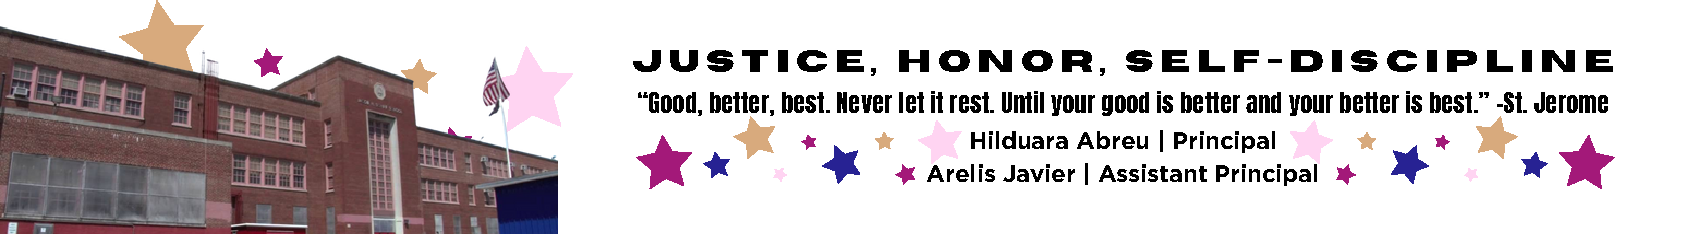
\includegraphics[width=8.8in,height=1.3in]{logo-1}}\end{picture}}
\fancyhead[C]{\setlength{\unitlength}{1in}\begin{picture}(5,0)\put(-1.9,-0.5){
\includegraphics[width=8.9in,height=1.3in]{logo-2}}\end{picture}}
\fancyhead[R]{\thepage}
\pagenumbering{gobble}

\begin{document}
\vspace*{0.1in}

Date: \href{https://www.ps192.org/apps/bbmessages/show_bbm.jsp?REC_ID=139439}{February 16, 2024}

Sujeto: Horario Escolar

Un horario escolar especifica la hora de inicio y la duración de uno o más períodos de instrucción de cada día. Un horario diario consistente y rutinario
les ofrece a los niños una disciplina de trabajo durante la semana de clase. Un
horario escolar ayuda a los niños a:
\begin{itemize}
\item Sentirse en control de su entorno.
\item Sentirse seguro, protegido y cómodo.
\item Poder realizar una actividad o tarea.
\item Participar en el aprendizaje.
\end{itemize}

Al igual que los adultos, los niños se sienten más confiados y seguros cuando sus
actividades diarias son predecibles y familiares.

\tcbuselibrary{}
\newtcolorbox{bluebox}[1][]{
  colback=blue!5!white,
  colframe=blue!75!black,
  fonttitle=\bfseries,
  coltitle=black,
  enhanced,
  attach boxed title to top center={yshift=-2mm},
  title=#1,
  boxed title style={colback=blue!50!white}
}
\newtcolorbox{greenbox}[1][]{
  colback=green!5!white,
  colframe=green!75!black,
  fonttitle=\bfseries,
  coltitle=black,
  enhanced,
  attach boxed title to top center={yshift=-2mm},
  title=#1,
  boxed title style={colback=green!50!white}
}
\newtcolorbox{redbox}[1][]{
  colback=red!5!white,
  colframe=red!75!black,
  fonttitle=\bfseries,
  coltitle=black,
  enhanced,
  attach boxed title to top center={yshift=-2mm},
  title=#1,
  boxed title style={colback=red!50!white}
}

\begin{bluebox}[PS 192 | Horario Escolar]
\begin{table}[H]
\centering
\begin{tblr}{
  colspec={|X|X|X|X|},
  row{1}={font=\bfseries\color{MacaroniandCheese},c},
  hlines,
  vlines,
  hline{1,10} = {-}{0.08em},
}
\textbf{Periodo} & \textbf{Hora de Inicio} & \textbf{Hora de Termino} & \textbf{Duración} \\
1               & 08:00 AM                & 08:45 AM                 & 45 minutos         \\
2               & 08:45 AM                & 09:30 AM                 & 45 minutos         \\
3               & 09:30 AM                & 10:15 AM                 & 45 minutos         \\
4               & 10:15 AM                & 11:05 AM                 & 50 minutos         \\
5               & 11:05 AM                & 11:55 AM                 & 50 minutos         \\
6               & 11:55 AM                & 12:40 PM                 & 45 minutos         \\
7               & 12:40 PM                & 01:30 PM                 & 50 minutos         \\
8               & 01:30 PM                & 02:15 PM                 & 45 minutos
\end{tblr}
\end{table}
\end{bluebox}
\end{document}
